\section{Motivating Example}

In this article we are discuss context-free constrained path quering, and one of well-known not regular but context-free language is an 
language $$\mathcal{L} = \{A^n B^n; n \geq 1\} = \{AB; AABB; AAABBB; \dots\}$$.
This language is a subset of balanced brackets langage and in practice may be used for description many different relations: n-th generation in parent-child, any open should be closed in correct order, etc.. 

As a motivation of context-free constraints importance let we introduce the next example.
Let we have graph $M=(\{0;1;2;3\},E,\{A;B\})$ presented in figure~\ref{input} where labels represent next relations:

each time when it opend it should be closed in future.

Suppose for each $n \geq 1$ we want to find all $n$-th generation friends with a common ancestor.
In the other worlds, we wath to find all paths $p$, such that $\Omega(p) \in \{AB; AABB; AAABBB; \dots\}$ or $\Omega(p) = A^n B^n$ where $n \geq 1$.
This constraint can not be specified with regular language as far as $L=\{A^n B^n; n \geq 1\}$ is not regular but context free.
Required language can be specified by grammar $G_1$ presented in picture~\ref{grammarG} where $N = \{s; middle\}$, $\Sigma = \{A; B\}$, and $S = s$.

\begin{figure}[h]
    \begin{center}
        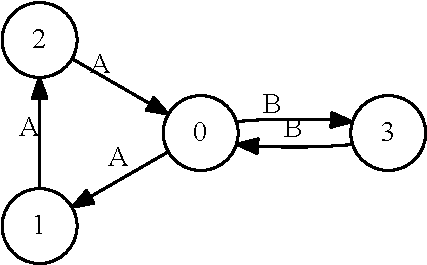
\includegraphics[width=6cm]{dot/input.pdf}
        \caption{Input graph $M$}
        \label{input}        
    \end{center}
\end{figure}

\begin{figure}[h]
   \begin{center}
\begin{verbatim}
   0: s = L s R 
   1: s = middle
   2: middle = L R
\end{verbatim}
   \caption{Grammar $G_1$ for language $L=\{L^n R^n; n \geq 1\}$}
   \label{grammarG}        
   \end{center}
\end{figure}


Result is infinite for this query, and we can not... 
Also we want to know, who is common accesor.
Futher we show ho to solve it.
